% This is the Reed College LaTeX thesis template. Most of the work
% for the document class was done by Sam Noble (SN), as well as this
% template. Later comments etc. by Ben Salzberg (BTS). Additional
% restructuring and APA support by Jess Youngberg (JY).
% Your comments and suggestions are more than welcome; please email
% them to cus@reed.edu
%
% See http://web.reed.edu/cis/help/latex.html for help. There are a
% great bunch of help pages there, with notes on
% getting started, bibtex, etc. Go there and read it if you're not
% already familiar with LaTeX.
%
% Any line that starts with a percent symbol is a comment.
% They won't show up in the document, and are useful for notes
% to yourself and explaining commands.
% Commenting also removes a line from the document;
% very handy for troubleshooting problems. -BTS

% As far as I know, this follows the requirements laid out in
% the 2002-2003 Senior Handbook. Ask a librarian to check the
% document before binding. -SN

%%
%% Preamble
%%
% \documentclass{<something>} must begin each LaTeX document
\documentclass[12pt,twoside]{reedthesis}
% Packages are extensions to the basic LaTeX functions. Whatever you
% want to typeset, there is probably a package out there for it.
% Chemistry (chemtex), screenplays, you name it.
% Check out CTAN to see: http://www.ctan.org/
%%
\usepackage{graphicx,latexsym}
\usepackage{amsmath}
\usepackage{amssymb,amsthm}
\usepackage{longtable,booktabs,setspace}
\usepackage{chemarr} %% Useful for one reaction arrow, useless if you're not a chem major
\usepackage[hyphens]{url}
% Added by CII
\usepackage{hyperref}
\usepackage{lmodern}
\usepackage{float}
\floatplacement{figure}{H}
% End of CII addition
\usepackage{rotating}

% Next line commented out by CII
%%% \usepackage{natbib}
% Comment out the natbib line above and uncomment the following two lines to use the new
% biblatex-chicago style, for Chicago A. Also make some changes at the end where the
% bibliography is included.
%\usepackage{biblatex-chicago}
%\bibliography{thesis}


% Added by CII (Thanks, Hadley!)
% Use ref for internal links
\renewcommand{\hyperref}[2][???]{\autoref{#1}}
\def\chapterautorefname{Chapter}
\def\sectionautorefname{Section}
\def\subsectionautorefname{Subsection}
% End of CII addition

% Added by CII
\usepackage{caption}
\captionsetup{width=5in}
% End of CII addition

% \usepackage{times} % other fonts are available like times, bookman, charter, palatino


% To pass between YAML and LaTeX the dollar signs are added by CII
\title{My Final College Paper}
\author{Wenxin Du}
% The month and year that you submit your FINAL draft TO THE LIBRARY (May or December)
\date{May 2020}
\division{Mathematics and Natural Sciences}
\advisor{Andrew Bray}
%If you have two advisors for some reason, you can use the following
% Uncommented out by CII
% End of CII addition

%%% Remember to use the correct department!
\department{Mathematics}
% if you're writing a thesis in an interdisciplinary major,
% uncomment the line below and change the text as appropriate.
% check the Senior Handbook if unsure.
%\thedivisionof{The Established Interdisciplinary Committee for}
% if you want the approval page to say "Approved for the Committee",
% uncomment the next line
%\approvedforthe{Committee}

% Added by CII
%%% Copied from knitr
%% maxwidth is the original width if it's less than linewidth
%% otherwise use linewidth (to make sure the graphics do not exceed the margin)
\makeatletter
\def\maxwidth{ %
  \ifdim\Gin@nat@width>\linewidth
    \linewidth
  \else
    \Gin@nat@width
  \fi
}
\makeatother

\renewcommand{\contentsname}{Table of Contents}
% End of CII addition

\setlength{\parskip}{0pt}

% Added by CII

\providecommand{\tightlist}{%
  \setlength{\itemsep}{0pt}\setlength{\parskip}{0pt}}

\Acknowledgements{
I want to thank a few people.
}

\Dedication{
You can have a dedication here if you wish.
}

\Preface{
This is an example of a thesis setup to use the reed thesis document
class (for LaTeX) and the R bookdown package, in general.
}

\Abstract{
The preface pretty much says it all. \par  Second paragraph of abstract
starts here.
}

% End of CII addition
%%
%% End Preamble
%%
%

\begin{document}

% Everything below added by CII
      \maketitle
  
  \frontmatter % this stuff will be roman-numbered
  \pagestyle{empty} % this removes page numbers from the frontmatter

      \begin{acknowledgements}
      I want to thank a few people.
    \end{acknowledgements}
  
      \begin{preface}
      This is an example of a thesis setup to use the reed thesis document
      class (for LaTeX) and the R bookdown package, in general.
    \end{preface}
  
      \hypersetup{linkcolor=black}
    \setcounter{tocdepth}{2}
    \tableofcontents
  
      \listoftables
  
      \listoffigures
  
      \begin{abstract}
      The preface pretty much says it all. \par  Second paragraph of abstract
      starts here.
    \end{abstract}
  
      \begin{dedication}
      You can have a dedication here if you wish.
    \end{dedication}
  
  \mainmatter % here the regular arabic numbering starts
  \pagestyle{fancyplain} % turns page numbering back on

  \chapter*{Introduction}\label{introduction}
  \addcontentsline{toc}{chapter}{Introduction}
  
  \chapter{SCA and Its Applications}\label{sca-and-its-applications}
  
  \par 
  
  It has come to researchers' attention that, the minor decisions made by
  researchers along the way of performing a data analysis can have a
  larger effect on the final research output than expected. A dataset can
  be analyzed in lots of different ways as there are a great number of
  decisions that can be made by a researcher: which statistical test to
  perform, which variables to include, which transformation to make on
  variables, etc. And by making specific decisions along the way, such as
  ``multiple comparison'', it is possible to find a p-value of less than
  0.05 on data with absolutely no relationship. This problem is often
  called ``p-hacking'' or ``researcher degrees of freedom''. A great
  number of recent studies looked into this problem closely, and it's been
  discovered that even if researchers are not consciously performing the
  action of ``p-hacking'', when the details in a data analysis are too
  contingent on data, there can still be the problem of multiple potential
  comparisons (cite Gelman and Loken 2013). It is now commonly realized
  that simply following the traditionally appropriate way to conduct a
  data analysis and look for a statistically significant p-value is no
  longer sufficient to produce reliable results.
  
  \par 
  
  The decisions made by a researcher, or in the other term, the
  specifications, are often a small subset of a much larger set of valid
  specifications. Thus there can be great limitation on the conclusiveness
  of the results, as the results usually hinge on the selected
  specifications, and sometimes the selection of specifications are made
  under researchers' hope to produce a publishable exciting story. Methods
  have been proposed to work around with the existence of such problem,
  and one approach taken in social science is to consider the robustness
  of models in response to alternative specifications. It is the
  consideration that, assuming some alternative sets of specifications
  were chosen by the researchers, how would the different results agree
  with each other. From there it is possible to get a sense of how greatly
  the original result hinges on the choices of specifications. The one
  method that will be focused on in this thesis is the Specification-curve
  analysis (SCA), proposed by Simonsohn, Simmons, Nelson in 2015. SCA
  considers non-overlapping sets of reasonble specifications and the
  potential different conclusions that one can arrive on. The method
  provides a way to visualize the different results one can arrive based
  on the different choices of specifications and to have a general
  understanding on where the differences may orginate from. Most
  importantly, it provides an assessment of a model's robustness in
  response to changes in specifications.
  
  \par 
  
  The few applications of SCA are all in the field of psychology. Several
  psychologists have applied this method on controversial topics which
  gather global attention. However, some usage of the method seens to be
  deviated from the original purpose of the method, and the conclusion
  drawn by the analysis remains questionable. One of the major application
  of SCA, the study of the association between adolescent well-being and
  digital technology use by Orben and Przybylski published on nature in
  2019, is one of such applications. After a full replication of Orben's
  study, it's found that the main problems of this study lie in the
  misunderstanding of the type of specifications that SCA works with, and
  the inference of the SCA result. The replication and details on the
  problems will be discussed in Chapter 2. In the following sections, we
  will introduce in details about SCA, its existing applications, and
  Orben's application.
  
  \par 
  
  (The thesis also focuses on\ldots{} formal inference method for SCA?
  Potential improvement of the method?)
  
  \section{Specification-Curve
  Analysis}\label{specification-curve-analysis}
  
  \par 
  
  Conducting a specification-curve analysis involves three steps: (1)
  Identifying set of specifications, (2) Estimate all specifications and
  construct a descriptive specification curve, (3) Conduct inferential
  analysis on a specification curve. This section discusses the details in
  each step, along with the important assumptions and concepts of the
  method.
  
  \subsection{Specifications}\label{specifications}
  
  \par 
  
  The first step of conducting a Specification-Curve Analysis is to
  enumerate the set of specifications to be considered.
  Specficiation-Curve Analysis focuses on a specific set of
  specifications: the set of specifications which are (1) consistent with
  the underlying theory, (2) expected to be statistically valid, (3) are
  not redundant with other specifications in the set. The specifications
  used in a SCA should be the valid and non-redundant specifications
  considered by the researcher. It is common that different researchers
  have disagreements over specifications, and when conducting a SCA, a
  researcher needs only to consider the set of valid specifications in
  their own perspective. If there are lots of overlaps between two
  researchers' sets of valid specifications, the results of two SCA's
  should be similar. If the two sets hardly or even never overlap, the
  results of two SCA's would be different. And such difference between
  analyses' results would most likely not be difference happening by
  chance, but may be originated by something fundamentally different,
  maybe different underlying theory.
  
  \par 
  
  One important concept about the Specification-Curve Analysis is that,
  the specifications considered in an SCA are all operationlization
  decisions, not theorizing decisions. Say we are conducting an SCA
  studying the relationship between Y and X. Some appropriate
  specifications to be used in an SCA can be, ``Do a log transformation on
  variable X'', ``Exclude these three outliers'', ``Include variable K as
  control variable'', ``Add an intersection term between X and K'', or
  ``Do a logit model instead of a probit model''. These specifications all
  focus on, after the underlying theory is determine and the statistical
  question has been stated, what type of operations I can do to my model
  that does not change the main characters in the story but may make small
  differences that can affect the story ending. But specifications that
  are based on different underlying theory are not the type of
  specifications that an SCA can work with. For example, if the question
  of interest is the relationship between class performance and hair
  color, where the hair color was intended to be the natural hair color
  that is determined by genes, using a variable that also considers dyed
  hair color would not be appropriate, since the action of dyeing hair
  reveals information regarding personalities, and the choice of hair
  coloring also reveals information regarding personalities. The
  relationship between this class performance and this variable will be
  telling a different story. It would thus not be appropriate in this case
  to consider the interchange of these two variables as an appropriate
  specification, as the underlying theories are different.
  
  \par 
  
  Note that sometimes the set of specifications can be huge and difficult
  to computationally work with. For example, say we are working on a
  dataset with 10 variables, and say we have: 1) 2 possible regression
  model, 2) 2 ways of transforming each of the 10 variables, 3) 3 ways for
  each variable to deal with outliers, and 4) 10 ways of adding
  interaction terms, this will result in 12000 different models to run
  with each model are built based on a different set of specifications.
  And in reality, the number of variables can be much larger than 10, and
  the model form can be much more complicated. In case if the set of
  specifications is too large, it was proposed that a random subset of the
  specifications can be used instead.
  
  \subsection{Specification Curve}\label{specification-curve}
  
  \par 
  
  The next step will be running estimation on the set of different models
  based on the enumerated specifications, and then constructing a
  specification curve. Shown below is an example of a specification curve
  (cite)
  
  \%\texttt{\{r\ SpecCurv,\ fig.cap="Specification\ Curve",\ fig.width=6\}\ \%include\_graphics(path\ =\ "figure/specificationCurve.png")\ \%}
  \% To be edited
  
  \par 
  
  As shown in the graph, a descriptive specification curve encompasses two
  parts: the top plot of a curve, and the bottom plot with lines and dots
  on it. The curve is the curve of the estimates from each of the model,
  ordered from lowest value to highest value. In the bottom half of the
  plot, each dot represents the usage of a specification. The vertical
  axis are the specifications used. And for each dot on the curve, there
  is a corresponding column in the bottom plot. If a specification was
  used in the model that produced this specific estimation, there will be
  a dot in the column at the position matching with the specification name
  on the vertical axis. Therefore, overall, it is possible to visualize if
  there exist certain pattern in choice of combination of specifications
  and the corresponding estimation. Also included on plot is the
  indication of the models with statistcially significant estimation. From
  the plot it is possible to visualize if the statistical significance
  appears to be happening purely by chance, or if there appears to be some
  real relationship. If so, if the relationship appears robust under
  changes in specifications.
  
  \subsection{Specification-Curve
  Analysis}\label{specification-curve-analysis-1}
  
  \par 
  
  The last step of a SCA is the statistical inference. The question for an
  inferential analysis, as stated by the authors, is ``\emph(Considering
  the full set of reasonable specifications jointly, how inconsistent are
  the results with the null hypothesis of no effect?)''. No step-by-step
  instructions are given for a complete inferential analysis. It was
  suggested that using the technique of resampling, one can generate an
  expected distribution of specification curves when the null hypothesis
  is true. The examples provided in the paper all used the permutation
  technique, while it was suggested that a bootstrapping technique is also
  applicable for studies without random assignment.
  
  \par 
  
  Three test statistics are proposed for the inferential analysis, but the
  authors do not specify which ones might be more favored: 1) the median
  overall point estimate from the specification curve, 2) the share of
  estimates in specification curve that are of the dominant sign, 3) the
  share that are of the dominant sign and also statistically significant
  (p \textless{} 0.05). The dominant sign here refer to the sign of the
  majority of estimates. If the majority of the estimates in a SCA have
  positive sign, then the dominant sign will be positive. Generally we
  would not expect half the estimates to be positive and the rest to be
  negative, as the different models are not fundamentally different but
  rather similar at most places. This test statistic performs as a summary
  of the entire specification curve, and the resampling procedure produces
  a null distribution of the test statistic. The p-value extracted, as
  claimed by the authors, will answer the inferential question we
  proposed. One thing worth noting is the interpretation of the p-value.
  In the examples listed in the paper, the actual numerical value of the
  test statistic are not meaningful. The p-value, however, indicates how
  robust the estimates are in response to changes in specifications. A low
  p-value indicates inconsistency with the null hypothesis of no effect,
  indicating strong sign for the existence of statistically significant
  relationship. A high p-value indicates consistency with the null
  hypothesis of no effect, suggesting the failure to reject the hypothesis
  that no relationship exist.
  
  \section{Applications of SCA}\label{applications-of-sca}
  
  \subsection{Existing applications}\label{existing-applications}
  
  \subsection{Orben's Application}\label{orbens-application}
  
  \chapter{Replication and Evaluation}\label{replication}
  
  This section discusses the attempt to replicate Orben's study along with
  the assessment of the use of SCA in this study. We begin by introducing
  the three datasets used, which can all be found through public sources
  under permission. We then discuss in details the attempt to replicate
  the study, including the obstacles to overcome during the replication
  process.
  
  \section{Data and Reprocessing}\label{data-and-reprocessing}
  
  \par 
  
  Three large-scale social datasets were used in Orben's study: Monitoring
  the Future (MTF) from the US {[}cite{]}, Youth Risk and Behavior Survey
  (YRBS) from the US {[}cite{]}, and Millennium Cohort Study (MCS) from
  the United Kingdom {[}cite{]}. The three datasets were all survey data
  obtained from scientific study of the same name, and encompass survey
  answers from adolescents aged predominately 12-18 in the time period of
  2007 to 2016. The datasets provided wide measures of adolescents'
  psychological well-being and digital technology use. A considerable
  number of psychology studies in the existing literature were conducted
  based on the large-scale studies, which provided wide selection of
  approaches to modeling and analysis based on the specific dataset. In
  this section, we discuss the background information of the three
  datasets and the reprocessing of the data obtained from public sources.
  
  \subsection{YRBS}\label{yrbs}
  
  \par 
  
  The Youth Risk Behavior Surveillance was first launched in 1990, and
  it's a biennial survey of adolescents that reflects a nationally
  representative sample of students attending secondary schools. Orben's
  study focused on the data collected during the time period of 2007 to
  2015, and the same set of data was obtained through (website
  name){[}cite{]}. While Orben used data in SPSS format, we were only able
  to access the data through Microsoft Access. The datasets were extracted
  and saved under excel format. It was confirmed that same number of
  observations were included in the obtained dataset as the data used by
  Orben, 37,402 girls and 37,412 boys from 2007 to 2015. It was also
  confirmed that all variables used in Orben's study are contained in the
  obtained dataset. Most of the work in the reprocessing step for YRBS
  focused on transforming the characteristic values of the variables used
  by Orben into relative numerical values.
  
  \par 
  
  One noticeable obstacle in this reprocessing step was, since the study
  is conducted anually and is still ongoing, the survey questions and
  indexings have been updated several times in the recent years. The
  majority of the variables in the datasets are named after the survey
  questions indexes, and the recent updates in survey questions result in
  differences of indices for survey questions between the current survey
  and surveys conducted prior to 2015. This lead to mismatches between
  variable names in the incorporated dataset including data from year of
  2015 and prior--the one used by Orben--and the variable names in the
  dataset obtained for this study, including data from the year of 2017
  and prior. Careful research and recoding are done to ensure the correct
  set of variables was used for the replication.
  
  \subsection{MTF}\label{mtf}
  
  \par 
  
  Monitoring the Future was first launched in the year of 1975, and it is
  an annual nationally representative survey of approximately 50,000 US
  adolescents in grades 8, 10 and 12. Surveys on adolescents in grade 12
  were not used in the analysis since ``many of the key items of interest
  cannot be correlated in their survey''. Orben focused on the data
  collected during the time period of 2008 to 2016, which included 136,190
  girls and 132,482 boys. The data are publicly accessible. In Orben's
  study, a merged dataset containing MTF data from 2008 to 2016 was used.
  While the MTF data for each year is publicly accessible, no access to a
  merged MTF dataset for the specified time period have been found. During
  the time period of 2008 to 2016, the survey has been updated multiple
  times, along with one major change in data file format after RStudio's
  release in the year of 2011. Due to the frequent updates in the annual
  surveys and changes in data files, the variable names vary greatly among
  the available datasets. This bring excessive difficulties to obtain the
  exact same dataset as used in Orben's study for replication purpose.
  
  \subsection{MCS}\label{mcs}
  
  \par 
  
  The Millennium Cohort Study follows a specific cohort of children born
  between September 2000 and January 2001 and collects data from both the
  children and the caregivers. Orben's study focused specifically on the
  data collected in 2015, when the participated children were aged between
  13 and 15. The sample included 5926 girls and 5946 boys along with 10605
  caregivers. The same dataset as used by Orben was obtained. The access
  to the data is open to public but require specific permission. While
  Orben obtained data in csv format, we were only able to obtain data in
  SPSS format. The same set of observations, with 5926 girls and 5946 boys
  borned between September 2000 and January 2001, were included in the
  dataset, along with the same set of variables as used in Orben's study.
  
  \par 
  
  Unlike working with YRBS and MTF, the variable names in the obtained
  dataset matches well with the variable names in the dataset used by
  Orben. However, instead of using numerical indices to represent survey
  answers, in the dataset obtained, the variable values were all in
  characters with the specific content refering to the specific survey
  answer. After careful reprocessing, all variable values were transformed
  into the exact numerical indices matching with the variables values as
  were in Orben's study. However, two variables--one related to family
  incomes and one related to siblings--had only NA values in the obtained
  dataset. The omissions might be done for confidential purpose. The two
  variables were used as control variables in Orben's study. As we fail to
  obtain the two variables, they were removed for this attempt to
  replication.
  
  \section{Replication}\label{replication}
  
  \par 
  
  After obtainning the datasets we began the replication of Orben's study.
  The replication consists of two parts, the replication of a single SCA
  analysis for each dataset, and the replication of the SCA permutation
  test, which was used by Orben to assess the significance of the single
  SCA result. In the following section we discuss the procedure, obstacles
  and the specific resolutions to the obstacles of replicating the
  analysis.
  
  \subsection{SCA}\label{sca}
  
  \par 
  
  The first part of the replication is to replicate the single SCA
  analysis for each dataset. All the replications in this section were
  done mostly by the original code provided by Orben in the public github
  repository. Due to the necessary reprocessings mentioned in the previous
  sections, slight modifications were made to the original code for the
  replication to be done smoothly.
  
  \par 
  
  It is important to understand what Orben considers as a
  ``specification'' and how a specification is identified in this study.
  \textbf{(Include a ``definition'' of specification here)} In this case,
  the model is set to be a linear regression, with a response variable
  representing ``adolescent mental well-being'' and an independent
  variable representing ``technology use'', with an optional set of other
  independent variable considered as control variables. An alternative
  speicification here is an alternative combination of variables to be
  used in the linear model. For example, one alternative specification may
  be using the variable ``amount of time spent on watching TV in a day''
  as the independent variable representing ``technology use'', ``number of
  times thought of suicide'' as the dependent variable representing
  ``adolescent mental well-being'', and a list of selected variables as
  control variables, while another alternative specification choose
  ``whether or not you own a personal computer at home'' as the
  independent variable representing ``technology use'' instead. An
  identified specification include one identified variable for
  ``technology use'', one identified variable for ``adolescent mental
  well-being'', and making the decision of whether or not to include
  control variables in the model (i.e.~simple linear regression or
  multivariate linear regression). The number of specifications determined
  vary among three datasets, as the number of relevant variables is
  different in different dataset.
  
  \par 
  
  Nearly 2.5 trillion alternative specifications were determined for the
  MCS study. Considering the computational ability, a random subset of
  20,004 specifications for the SCA analysis on MCS data was used instead.
  A seed is not provided by Orben for the random subset, thus we failed to
  obtain the exact same subset of specification for this SCA analysis. We
  instead randomly generated our own subset of 20,004 specifications. It
  is noteworthy that this randomness can result in discrepancy in SCA
  result. Considering that the random subset has large size, we expect the
  degree of this discrepancy to be small. And this expectation is
  confirmed by replication result: while Orben obtained the median
  coefficient of the independent variable to be
  \(Median(\beta) = -0.032\), our replication obtained
  \(Median(\beta) = -0.0328\).
  
  \par 
  
  The problem does not exist for the studies YRBS and MTF. There were less
  variables available in the dataset relating to technology use and
  adolescent mental well-being. The number of specifications identified in
  the two studies are in reasonable size, therefore the exact set of
  specifications were used for the replications. The result matched well
  with Orben's result. The median coefficient of the independent variable
  in the YRBS study was found to be \(Median(\beta) = -0.035\) in Orben's
  study. The result obtained in this replication, when rounded to the same
  digits, is also -0.035.
  
  \par 
  
  \textbf{MTF to be discussed}
  
  \subsection{Bootstrapping test}\label{bootstrapping-test}
  
  \par 
  
  The next part of the replication is to replicate the inference of the
  single specification curves for each data. Orben chose to use a
  bootstrapping test on the median overall point estimate for significance
  of the result. We will later assess the choice of the inference test and
  the correctness of the inference. For now, we will focus mainly on
  replicating the process to conduct the bootstrapping test as Orben did
  and the attempt to replicate her result.
  
  \par 
  
  500 SCA tests were conducted in Orben's study on bootstrapped samples
  for each of the three datasets, and the single SCA results were shown to
  be significant for all three datasets. The code for the bootstrapping
  test and SCA are all publically available on Orben's github repository
  {[}cite{]}. The initial attempt of the replication was done using the
  original code. However, due to the large sizes of the three datasets and
  the great number of loops used in the R code, the replication process
  becomes computational expensive. A single SCA will take around 8 hours
  to run, and performing 500 SCA will take nearly 24 weeks. An ARC
  computer cluster at Oxford was used by Orben to reduce running time,
  however, no access to such advanced computer is available for this
  replication. Therefore, instead of using purely the original code, the
  code for single SCA and bootstrapping distribution of SCA results have
  been rewritten using parallel running. The running time have been
  significantly reduced. The dataset YRBS has the least number of
  observations and specifications, and after the recoding it now takes
  about 9 hours for a complete boostrapping test with 500 SCA's to be done
  using a computer with 8 cores. More time will be needed for the other
  two datasets, as the number of observations and specifications can be
  much higher in those two cases. A 96-core server is used.
  \textbf{Detail times should be added later}
  
  \section{Evaluating Orben's work}\label{evaluating-orbens-work}
  
  The replication of Orben's work allows a better understanding of Orben's
  approach and procedure. As mentioned in previous chapter, there exists a
  number of errors in this study in terms of the usage of SCA, including
  fundamental misunderstanding of the intentionals of the SCA method,
  inappropriate choice of specifications, and misinterpretation of the SCA
  results.
  
  \subsection{\texorpdfstring{``one-to-many'' mapping from scientific to
  statistical
  hypotheses}{one-to-many mapping from scientific to statistical hypotheses}}\label{one-to-many-mapping-from-scientific-to-statistical-hypotheses}
  
  \begin{itemize}
  \tightlist
  \item
    Choice of variable for ``tech'' - different variable different story,
    different underlying theories (- Choice of variable for
    ``well-being'')
  \end{itemize}
  
  \subsection{True SCA inference}\label{true-sca-inference}
  
  \begin{itemize}
  \tightlist
  \item
    Interpreting the actual numerical value of SCA test statistic? No,
    this is not how the SCA results should be interpreted. It only shows
    evidence for the existence of a relationship or not.
  \end{itemize}
  
  \subsection{Bootstrapping?
  Permutation?}\label{bootstrapping-permutation}
  
  \subsection{Choice of Multi-variate Linear
  Regression}\label{choice-of-multi-variate-linear-regression}
  
  \chapter{Tables, Graphics, References, and Labels}\label{ref-labels}
  
  \section{Tables}\label{tables}
  
  In addition to the tables that can be automatically generated from a
  data frame in \textbf{R} that you saw in {[}R Markdown Basics{]} using
  the \texttt{kable} function, you can also create tables using
  \emph{pandoc}. (More information is available at
  \url{http://pandoc.org/README.html\#tables}.) This might be useful if
  you don't have values specifically stored in \textbf{R}, but you'd like
  to display them in table form. Below is an example. Pay careful
  attention to the alignment in the table and hyphens to create the rows
  and columns.
  
  \begin{longtable}[]{@{}ccc@{}}
  \caption{\label{tab:inher} Correlation of Inheritance Factors for Parents
  and Child}\tabularnewline
  \toprule
  \begin{minipage}[b]{0.29\columnwidth}\centering\strut
  Factors\strut
  \end{minipage} & \begin{minipage}[b]{0.47\columnwidth}\centering\strut
  Correlation between Parents \& Child\strut
  \end{minipage} & \begin{minipage}[b]{0.16\columnwidth}\centering\strut
  Inherited\strut
  \end{minipage}\tabularnewline
  \midrule
  \endfirsthead
  \toprule
  \begin{minipage}[b]{0.29\columnwidth}\centering\strut
  Factors\strut
  \end{minipage} & \begin{minipage}[b]{0.47\columnwidth}\centering\strut
  Correlation between Parents \& Child\strut
  \end{minipage} & \begin{minipage}[b]{0.16\columnwidth}\centering\strut
  Inherited\strut
  \end{minipage}\tabularnewline
  \midrule
  \endhead
  \begin{minipage}[t]{0.29\columnwidth}\centering\strut
  Education\strut
  \end{minipage} & \begin{minipage}[t]{0.47\columnwidth}\centering\strut
  -0.49\strut
  \end{minipage} & \begin{minipage}[t]{0.16\columnwidth}\centering\strut
  Yes\strut
  \end{minipage}\tabularnewline
  \begin{minipage}[t]{0.29\columnwidth}\centering\strut
  Socio-Economic Status\strut
  \end{minipage} & \begin{minipage}[t]{0.47\columnwidth}\centering\strut
  0.28\strut
  \end{minipage} & \begin{minipage}[t]{0.16\columnwidth}\centering\strut
  Slight\strut
  \end{minipage}\tabularnewline
  \begin{minipage}[t]{0.29\columnwidth}\centering\strut
  Income\strut
  \end{minipage} & \begin{minipage}[t]{0.47\columnwidth}\centering\strut
  0.08\strut
  \end{minipage} & \begin{minipage}[t]{0.16\columnwidth}\centering\strut
  No\strut
  \end{minipage}\tabularnewline
  \begin{minipage}[t]{0.29\columnwidth}\centering\strut
  Family Size\strut
  \end{minipage} & \begin{minipage}[t]{0.47\columnwidth}\centering\strut
  0.18\strut
  \end{minipage} & \begin{minipage}[t]{0.16\columnwidth}\centering\strut
  Slight\strut
  \end{minipage}\tabularnewline
  \begin{minipage}[t]{0.29\columnwidth}\centering\strut
  Occupational Prestige\strut
  \end{minipage} & \begin{minipage}[t]{0.47\columnwidth}\centering\strut
  0.21\strut
  \end{minipage} & \begin{minipage}[t]{0.16\columnwidth}\centering\strut
  Slight\strut
  \end{minipage}\tabularnewline
  \bottomrule
  \end{longtable}
  
  We can also create a link to the table by doing the following: Table
  \ref{tab:inher}. If you go back to {[}Loading and exploring data{]} and
  look at the \texttt{kable} table, we can create a reference to this max
  delays table too: Table \ref{tab:maxdelays}. The addition of the
  \texttt{(\textbackslash{}\#tab:inher)} option to the end of the table
  caption allows us to then make a reference to Table
  \texttt{\textbackslash{}@ref(tab:label)}. Note that this reference could
  appear anywhere throughout the document after the table has appeared.
  
  \clearpage
  
  \section{Figures}\label{figures}
  
  If your thesis has a lot of figures, \emph{R Markdown} might behave
  better for you than that other word processor. One perk is that it will
  automatically number the figures accordingly in each chapter. You'll
  also be able to create a label for each figure, add a caption, and then
  reference the figure in a way similar to what we saw with tables
  earlier. If you label your figures, you can move the figures around and
  \emph{R Markdown} will automatically adjust the numbering for you. No
  need for you to remember! So that you don't have to get too far into
  LaTeX to do this, a couple \textbf{R} functions have been created for
  you to assist. You'll see their use below.
  
  In the \textbf{R} chunk below, we will load in a picture stored as
  \texttt{reed.jpg} in our main directory. We then give it the caption of
  ``Reed logo'', the label of ``reedlogo'', and specify that this is a
  figure. Make note of the different \textbf{R} chunk options that are
  given in the R Markdown file (not shown in the knitted document).
  
  \begin{Shaded}
  \begin{Highlighting}[]
  \KeywordTok{include_graphics}\NormalTok{(}\DataTypeTok{path =} \StringTok{"figure/reed.jpg"}\NormalTok{)}
  \end{Highlighting}
  \end{Shaded}
  
  \begin{figure}
  
\includegraphics[width=3.47in]{figure/reed} \caption{Reed logo}\label{fig:reedlogo}
  \end{figure}
  
  Here is a reference to the Reed logo: Figure \ref{fig:reedlogo}. Note
  the use of the \texttt{fig:} code here. By naming the \textbf{R} chunk
  that contains the figure, we can then reference that figure later as
  done in the first sentence here. We can also specify the caption for the
  figure via the R chunk option \texttt{fig.cap}.
  
  \clearpage 
  
  Below we will investigate how to save the output of an \textbf{R} plot
  and label it in a way similar to that done above. Recall the
  \texttt{flights} dataset from Chapter \ref{rmd-basics}. (Note that we've
  shown a different way to reference a section or chapter here.) We will
  next explore a bar graph with the mean flight departure delays by
  airline from Portland for 2014. Note also the use of the \texttt{scale}
  parameter which is discussed on the next page.
  
  \begin{Shaded}
  \begin{Highlighting}[]
  \NormalTok{flights }\OperatorTok\StringTok{ }\KeywordTok{group_by}\NormalTok{(carrier) }\OperatorTok
  \StringTok{  }\KeywordTok{summarize}\NormalTok{(}\DataTypeTok{mean_dep_delay =} \KeywordTok{mean}\NormalTok{(dep_delay)) }\OperatorTok
  \StringTok{  }\KeywordTok{ggplot}\NormalTok{(}\KeywordTok{aes}\NormalTok{(}\DataTypeTok{x =}\NormalTok{ carrier, }\DataTypeTok{y =}\NormalTok{ mean_dep_delay)) }\OperatorTok{+}
  \StringTok{  }\KeywordTok{geom_bar}\NormalTok{(}\DataTypeTok{position =} \StringTok{"identity"}\NormalTok{, }\DataTypeTok{stat =} \StringTok{"identity"}\NormalTok{, }\DataTypeTok{fill =} \StringTok{"red"}\NormalTok{)}
  \end{Highlighting}
  \end{Shaded}
  
  \begin{figure}
  \centering
  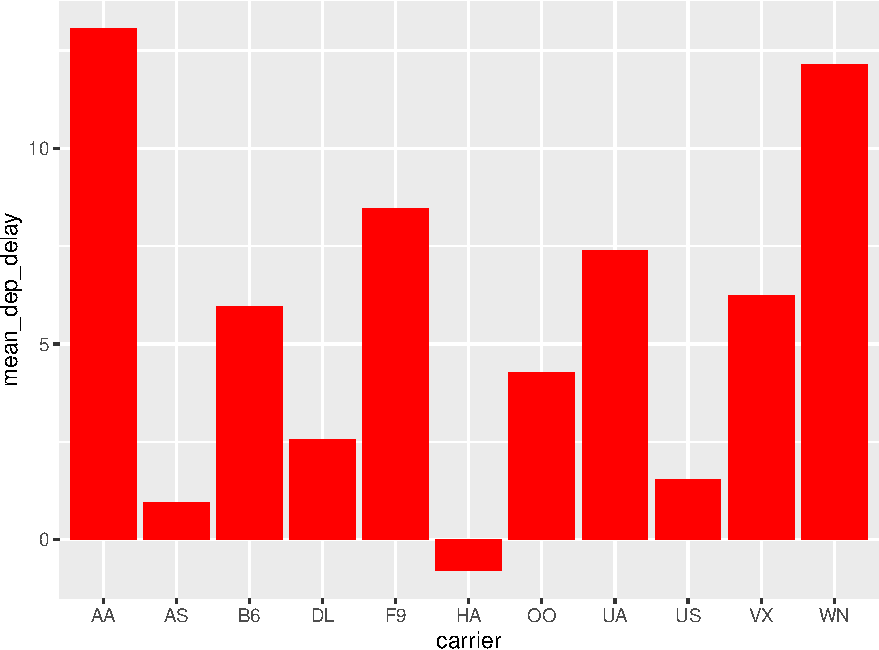
\includegraphics{thesis_files/figure-latex/delaysboxplot-1.pdf}
  \caption{\label{fig:delaysboxplot}Mean Delays by Airline}
  \end{figure}
  
  Here is a reference to this image: Figure \ref{fig:delaysboxplot}.
  
  A table linking these carrier codes to airline names is available at
  \url{https://github.com/ismayc/pnwflights14/blob/master/data/airlines.csv}.
  
  \clearpage
  
  Next, we will explore the use of the \texttt{out.extra} chunk option,
  which can be used to shrink or expand an image loaded from a file by
  specifying \texttt{"scale=\ "}. Here we use the mathematical graph
  stored in the ``subdivision.pdf'' file.
  
  \begin{figure}
  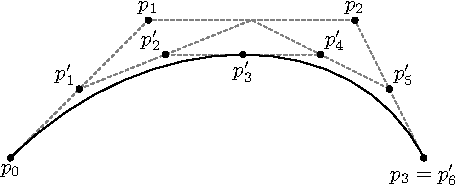
\includegraphics[scale=0.75]{figure/subdivision} \caption{Subdiv. graph}\label{fig:subd}
  \end{figure}
  
  Here is a reference to this image: Figure \ref{fig:subd}. Note that
  \texttt{echo=FALSE} is specified so that the \textbf{R} code is hidden
  in the document.
  
  \textbf{More Figure Stuff}
  
  Lastly, we will explore how to rotate and enlarge figures using the
  \texttt{out.extra} chunk option. (Currently this only works in the PDF
  version of the book.)
  
  \begin{figure}
  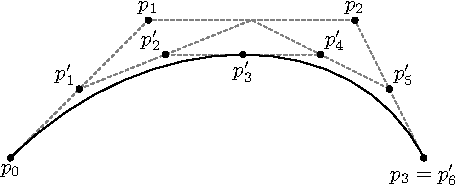
\includegraphics[angle=180, scale=1.1]{figure/subdivision} \caption{A Larger Figure, Flipped Upside Down}\label{fig:subd2}
  \end{figure}
  
  As another example, here is a reference: Figure \ref{fig:subd2}.
  
  \section{Footnotes and Endnotes}\label{footnotes-and-endnotes}
  
  You might want to footnote something.\footnote{footnote text} The
  footnote will be in a smaller font and placed appropriately. Endnotes
  work in much the same way. More information can be found about both on
  the CUS site or feel free to reach out to
  \href{mailto:data@reed.edu}{\nolinkurl{data@reed.edu}}.
  
  \section{Bibliographies}\label{bibliographies}
  
  Of course you will need to cite things, and you will probably accumulate
  an armful of sources. There are a variety of tools available for
  creating a bibliography database (stored with the .bib extension). In
  addition to BibTeX suggested below, you may want to consider using the
  free and easy-to-use tool called Zotero. The Reed librarians have
  created Zotero documentation at
  \url{http://libguides.reed.edu/citation/zotero}. In addition, a tutorial
  is available from Middlebury College at
  \url{http://sites.middlebury.edu/zoteromiddlebury/}.
  
  \emph{R Markdown} uses \emph{pandoc} (\url{http://pandoc.org/}) to build
  its bibliographies. One nice caveat of this is that you won't have to do
  a second compile to load in references as standard LaTeX requires. To
  cite references in your thesis (after creating your bibliography
  database), place the reference name inside square brackets and precede
  it by the ``at'' symbol. For example, here's a reference to a book about
  worrying: (Molina \& Borkovec, 1994). This \texttt{Molina1994} entry
  appears in a file called \texttt{thesis.bib} in the \texttt{bib} folder.
  This bibliography database file was created by a program called BibTeX.
  You can call this file something else if you like (look at the YAML
  header in the main .Rmd file) and, by default, is to placed in the
  \texttt{bib} folder.
  
  For more information about BibTeX and bibliographies, see our CUS site
  (\url{http://web.reed.edu/cis/help/latex/index.html})\footnote{Reed~College
    (2007)}. There are three pages on this topic: \emph{bibtex} (which
  talks about using BibTeX, at
  \url{http://web.reed.edu/cis/help/latex/bibtex.html}),
  \emph{bibtexstyles} (about how to find and use the bibliography style
  that best suits your needs, at
  \url{http://web.reed.edu/cis/help/latex/bibtexstyles.html}) and
  \emph{bibman} (which covers how to make and maintain a bibliography by
  hand, without BibTeX, at
  \url{http://web.reed.edu/cis/help/latex/bibman.html}). The last page
  will not be useful unless you have only a few sources.
  
  If you look at the YAML header at the top of the main .Rmd file you can
  see that we can specify the style of the bibliography by referencing the
  appropriate csl file. You can download a variety of different style
  files at \url{https://www.zotero.org/styles}. Make sure to download the
  file into the csl folder.
  
  \textbf{Tips for Bibliographies}
  
  \begin{itemize}
  \tightlist
  \item
    Like with thesis formatting, the sooner you start compiling your
    bibliography for something as large as thesis, the better. Typing in
    source after source is mind-numbing enough; do you really want to do
    it for hours on end in late April? Think of it as procrastination.
  \item
    The cite key (a citation's label) needs to be unique from the other
    entries.
  \item
    When you have more than one author or editor, you need to separate
    each author's name by the word ``and'' e.g.
    \texttt{Author\ =\ \{Noble,\ Sam\ and\ Youngberg,\ Jessica\},}.
  \item
    Bibliographies made using BibTeX (whether manually or using a manager)
    accept LaTeX markup, so you can italicize and add symbols as
    necessary.
  \item
    To force capitalization in an article title or where all lowercase is
    generally used, bracket the capital letter in curly braces.
  \item
    You can add a Reed Thesis citation\footnote{Noble (2002)} option. The
    best way to do this is to use the phdthesis type of citation, and use
    the optional ``type'' field to enter ``Reed thesis'' or
    ``Undergraduate thesis.''
  \end{itemize}
  
  \section{Anything else?}\label{anything-else}
  
  If you'd like to see examples of other things in this template, please
  contact the Data @ Reed team (email
  \href{mailto:data@reed.edu}{\nolinkurl{data@reed.edu}}) with your
  suggestions. We love to see people using \emph{R Markdown} for their
  theses, and are happy to help.
  
  \chapter*{Conclusion}\label{conclusion}
  \addcontentsline{toc}{chapter}{Conclusion}
  
  If we don't want Conclusion to have a chapter number next to it, we can
  add the \texttt{\{-\}} attribute.
  
  \textbf{More info}
  
  And here's some other random info: the first paragraph after a chapter
  title or section head \emph{shouldn't be} indented, because indents are
  to tell the reader that you're starting a new paragraph. Since that's
  obvious after a chapter or section title, proper typesetting doesn't add
  an indent there.
  
  \appendix
  
  \chapter{The First Appendix}\label{the-first-appendix}
  
  This first appendix includes all of the R chunks of code that were
  hidden throughout the document (using the \texttt{include\ =\ FALSE}
  chunk tag) to help with readibility and/or setup.
  
  \textbf{In the main Rmd file}
  
  \begin{Shaded}
  \begin{Highlighting}[]
  \CommentTok{# This chunk ensures that the thesisdown package is}
  \CommentTok{# installed and loaded. This thesisdown package includes}
  \CommentTok{# the template files for the thesis.}
  \ControlFlowTok{if}\NormalTok{(}\OperatorTok{!}\KeywordTok{require}\NormalTok{(devtools))}
    \KeywordTok{install.packages}\NormalTok{(}\StringTok{"devtools"}\NormalTok{, }\DataTypeTok{repos =} \StringTok{"http://cran.rstudio.com"}\NormalTok{)}
  \ControlFlowTok{if}\NormalTok{(}\OperatorTok{!}\KeywordTok{require}\NormalTok{(thesisdown))}
  \NormalTok{  devtools}\OperatorTok{::}\KeywordTok{install_github}\NormalTok{(}\StringTok{"ismayc/thesisdown"}\NormalTok{)}
  \KeywordTok{library}\NormalTok{(thesisdown)}
  \end{Highlighting}
  \end{Shaded}
  
  \textbf{In Chapter \ref{ref-labels}:}
  
  \begin{Shaded}
  \begin{Highlighting}[]
  \CommentTok{# This chunk ensures that the thesisdown package is}
  \CommentTok{# installed and loaded. This thesisdown package includes}
  \CommentTok{# the template files for the thesis and also two functions}
  \CommentTok{# used for labeling and referencing}
  \ControlFlowTok{if}\NormalTok{(}\OperatorTok{!}\KeywordTok{require}\NormalTok{(devtools))}
    \KeywordTok{install.packages}\NormalTok{(}\StringTok{"devtools"}\NormalTok{, }\DataTypeTok{repos =} \StringTok{"http://cran.rstudio.com"}\NormalTok{)}
  \ControlFlowTok{if}\NormalTok{(}\OperatorTok{!}\KeywordTok{require}\NormalTok{(dplyr))}
      \KeywordTok{install.packages}\NormalTok{(}\StringTok{"dplyr"}\NormalTok{, }\DataTypeTok{repos =} \StringTok{"http://cran.rstudio.com"}\NormalTok{)}
  \ControlFlowTok{if}\NormalTok{(}\OperatorTok{!}\KeywordTok{require}\NormalTok{(ggplot2))}
      \KeywordTok{install.packages}\NormalTok{(}\StringTok{"ggplot2"}\NormalTok{, }\DataTypeTok{repos =} \StringTok{"http://cran.rstudio.com"}\NormalTok{)}
  \ControlFlowTok{if}\NormalTok{(}\OperatorTok{!}\KeywordTok{require}\NormalTok{(ggplot2))}
      \KeywordTok{install.packages}\NormalTok{(}\StringTok{"bookdown"}\NormalTok{, }\DataTypeTok{repos =} \StringTok{"http://cran.rstudio.com"}\NormalTok{)}
  \ControlFlowTok{if}\NormalTok{(}\OperatorTok{!}\KeywordTok{require}\NormalTok{(thesisdown))\{}
    \KeywordTok{library}\NormalTok{(devtools)}
  \NormalTok{  devtools}\OperatorTok{::}\KeywordTok{install_github}\NormalTok{(}\StringTok{"ismayc/thesisdown"}\NormalTok{)}
  \NormalTok{  \}}
  \KeywordTok{library}\NormalTok{(thesisdown)}
  \NormalTok{flights <-}\StringTok{ }\KeywordTok{read.csv}\NormalTok{(}\StringTok{"data/flights.csv"}\NormalTok{)}
  \end{Highlighting}
  \end{Shaded}
  
  \chapter{The Second Appendix, for
  Fun}\label{the-second-appendix-for-fun}
  
  \backmatter
  
  \chapter*{References}\label{references}
  \addcontentsline{toc}{chapter}{References}
  
  \noindent
  
  \setlength{\parindent}{-0.20in} \setlength{\leftskip}{0.20in}
  \setlength{\parskip}{8pt}
  
  \hypertarget{refs}{}
  \hypertarget{ref-angel2000}{}
  Angel, E. (2000). \emph{Interactive computer graphics : A top-down
  approach with opengl}. Boston, MA: Addison Wesley Longman.
  
  \hypertarget{ref-angel2001}{}
  Angel, E. (2001a). \emph{Batch-file computer graphics : A bottom-up
  approach with quicktime}. Boston, MA: Wesley Addison Longman.
  
  \hypertarget{ref-angel2002a}{}
  Angel, E. (2001b). \emph{Test second book by angel}. Boston, MA: Wesley
  Addison Longman.
  
  \hypertarget{ref-Molina1994}{}
  Molina, S. T., \& Borkovec, T. D. (1994). The Penn State worry
  questionnaire: Psychometric properties and associated characteristics.
  In G. C. L. Davey \& F. Tallis (Eds.), \emph{Worrying: Perspectives on
  theory, assessment and treatment} (pp. 265--283). New York: Wiley.
  
  \hypertarget{ref-noble2002}{}
  Noble, S. G. (2002). \emph{Turning images into simple line-art}
  (Undergraduate thesis). Reed College.
  
  \hypertarget{ref-reedweb2007}{}
  Reed~College. (2007, March). LaTeX your document. Retrieved from
  \url{http://web.reed.edu/cis/help/LaTeX/index.html}


  % Index?

\end{document}

